\documentclass[a4paper]{article}

\usepackage[italian]{babel}
\usepackage[utf8]{inputenc}
\usepackage[T1]{fontenc}
\usepackage{enumitem}
\usepackage{graphicx}
\usepackage{float}
\usepackage{longtable}
\usepackage[table]{xcolor}
\usepackage{geometry}

\usepackage{lastpage}
\usepackage[bottom]{footmisc}
\usepackage{fancyhdr}
\usepackage{tabu}

\usepackage{pgffor}
\usepackage{etoolbox}
\usepackage{multirow}



\usepackage[official]{eurosym}

% Navigazione pdf
\usepackage{hyperref}
\hypersetup{
	colorlinks=true,
	linkcolor=black,
	filecolor=magenta,      
	urlcolor=blue,
}

\usepackage{tabularx}

\usepackage{multicol}
\newcommand{\glo}{\textsubscript{\emph{G}}}
\newcommand\hd{\emph{HD Viz}}
\newcommand\cod{\emph{Code of Duty}}
\newcommand{\myparagraph}[1]{\paragraph{#1}\mbox{}\\}
\newcommand{\mysubparagraph}[1]{\subparagraph{#1}\mbox{}\\}

\newcommand{\NdP}{\emph{Norme di Progetto 3.0.0}}
\newcommand{\PdP}{\emph{Piano di Progetto 3.0.0}}
\newcommand{\AdR}{\emph{Analisi dei requisiti 3.0.0}}
\newcommand{\PdQ}{\emph{Piano di Qualifica 3.0.0}}

\definecolor{header}{HTML}{FA8D21}
\definecolor{pari}{HTML}{DBDBDB}
\definecolor{dispari}{HTML}{F5F5F5}

\setcounter{secnumdepth}{4}

\pagestyle{fancy}
\lhead{
\includegraphics[scale=0.06]{../_template/images/logo_crop.png}}

%Titolo del documento
\rhead{\titolodocumento{}}
\cfoot{Pagina \thepage\ di \pageref{LastPage}}
\renewcommand{\footrulewidth}{0.4pt}

\newcommand{\titolodocumento}{Analisi dei requisiti} % Titolo documento
\newcommand{\versione}{ 2.3.0 } % Versione documento
\newcommand{\approvazione}{ Diego Piola } % Responsabile di progetto
\newcommand{\redazione}{\parbox[t]{4cm} {Andrea Mascari\\Damiano Zanardo\\Diego Piola\\}} % Redattori di questo documento
\newcommand{\verifica}{\parbox[t]{4cm} {Andrea Mascari\\Damiano Zanardo \\ Diego Piola \\ Alessandro Flori \\ } } % Verificatori di questo documento
\newcommand{\stato}{In lavorazione} % Approvato 
\newcommand{\uso}{Esterno} % Interno - Esterno
\newcommand{\destinazione}{\parbox[t]{4cm}{Prof Tullio Vardanega \\ Prof. Riccardo Cardin} } % Destinatario ( D1\\D2\\D3 )
\newcommand{\descrizionedocumento}{Il documento elenca casi d'uso e requisiti del progetto } % Descrizione documento

% Mettere sempre la virgola dopo l'ultima riga, se no si rompe la tabella

\def\modifiche{
    {v0.0.1, 02/12/2020, Damiano Zanardo, Analista , Prima bozza{,} aggiunti tutti i capitolati},
}



% Per modificare il frontespizio e diario delle modifiche andare sulla cartella source
% Per aggiungere il contenuto andare sulla cartella source/sections e creare un nuovo file.tex per ogni sezione

% Per parole che devono andare nel glossario aggiungere /glo{} dopo la parola

\begin{document}
    % Frontespizio 
    %\documentclass[a4paper]{article}
%\usepackage[italian]{babel}
\usepackage[utf8]{inputenc}
\usepackage[T1]{fontenc}
\usepackage{enumitem}
\usepackage{graphicx}
\usepackage{float}
\usepackage{longtable}
\usepackage[table]{xcolor}
\usepackage{geometry}

\usepackage{lastpage}
\usepackage[bottom]{footmisc}
\usepackage{fancyhdr}
\usepackage{tabu}

\usepackage{pgffor}
\usepackage{etoolbox}
\usepackage{multirow}



\usepackage[official]{eurosym}

% Navigazione pdf
\usepackage{hyperref}
\hypersetup{
	colorlinks=true,
	linkcolor=black,
	filecolor=magenta,      
	urlcolor=blue,
}

\usepackage{tabularx}

\usepackage{multicol}
%\begin{document}

\begin{titlepage}

	\begin{center}
		
\includegraphics[scale = 0.5]{../_template/images/logo.png}\\
		\large \textbf{Code of Duty - Progetto \emph{HD VIZ}} \\
		\vfill
		\huge \textbf{\titolodocumento}
		\vspace*{\fill}
        
        \vfill
        \large
    \end{center}
    
	\begin{table}[htbp]
        \centering
        \begin{tabular}{r|l}
            \textbf{Versione} & \versione{} \\
            \textbf{Approvazione} & \approvazione{} \\
            \textbf{Redazione} & \redazione{} \\
            \textbf{Verifica} & \verifica{} \\
            \textbf{Stato} & \stato{} \\
            \textbf{Uso} & \uso{} \\
            \textbf{Destinato a} & \destinazione{}
        \end{tabular}
    \end{table}
    
    \begin{center}
        \vfill
        \normalsize
        \textbf{Descrizione}\\
		\descrizionedocumento
        \vfill
        \small
        \texttt{info@codeofduty.it}
	\end{center}
\end{titlepage}

%\end{document}

    
    % Diario delle modifiche
    \newcommand*\mytablecontents{}
\foreach \x [count=\nj] in \modifiche
{
    \foreach \y [count=\ni] in \x
    {
        \ifnum\ni=6
            \xappto\mytablecontents{\y}
            \gappto\mytablecontents{\\}
            \gappto\mytablecontents{\hline}
        \else
            \xappto\mytablecontents{\y&}
        \fi
    }
}

\section*{Diario delle modifiche}

% Impostazioni della tabella
\tabulinesep = 2mm % padding
\taburowcolors [1] 2{pari .. dispari} % colori delle righe
\begin{longtabu} to \textwidth {| X[0.3, c m] | X[0.6,c m] | X[0.7,c m] | X[0.9,c m] | X[0.7,c m] | X[1.2,l m]|} % larghezza delle colonne
\hline
\rowcolor{header} % colore dell'header

\textbf{Ver.} & \textbf{Data} & \textbf{Nominativo} & \textbf{Ruolo} & \textbf{Verificatore} & \multicolumn{1}{c|}{\textbf{Descrizione}}\\
\hline
\mytablecontents

\end{longtabu}

    \pagebreak
    
    % Indice
    \tableofcontents
    \pagebreak
    
    % Se necessari
    % \listoffigures
    % \listoftables
    
    % Contenuto
    \section{Preventivo}
Nel Preventivo è indicata la divisione delle ore per ogni fase individuata nella sezione 4 del presente documento, insieme al prospetto economico. All'interno del Riepilogo è presentato il costo totale preventivato. Il tutto è corredato da diagrammi esemplificativi.
Si noti che nelle tabelle sono state utilizzate delle sigle, definite nelle \NdP . % mi porto avanti con le versioni
\subsection{Analisi}

    \subsubsection{Prospetto orario}
    %startTable
    \def\hourlycontent{
        {Andrea Breggion,6,14,3,0,0,6,29},
        {Matteo Falsetti,0,5,3,10,0,11,29},
        {Alessandro Flori,2,4,3,8,0,12,29},
        {Andrea Mascari,0,0,14,2,0,13,29},
        {Diego Piola,6,13,3,0,0,7,29},
        {Andrea Signori,12,6,4,0,0,7,29},
        {Damiano Zanardo,0,7,14,0,0,8,29},
        {Ore totali, 25, 51, 44, 19, 0, 64, 203},
    }
    %endTable
    \newcommand*\hourlysummary{}
\foreach \x [count=\nj] in \hourlycontent
{
    \foreach \y [count=\ni] in \x
    {
        \ifnum\ni=8
            \xappto\hourlysummary{\y}
            \gappto\hourlysummary{\\}
            \gappto\hourlysummary{\hline}
        \else
            \xappto\hourlysummary{\y&}
        \fi
    }
}

% Impostazioni della tabella
\tabulinesep = 2mm % padding
\taburowcolors [1] 2{pari .. dispari} % colori delle righe
\begin{longtabu} to \textwidth {| X[0.3, c m] | X[0.1, c m] | X[0.1, c m] | X[0.1, c m] | X[0.1, c m] | X[0.1, c m] | X[0.1, c m] | X[0.1, c m] |}
\hline
\rowcolor{header} % colore dell'header
\textbf{Membro} &
\textbf{Re} & 
\textbf{Ad} & 
\textbf{An} & 
\textbf{Pt} & 
\textbf{Pr} & 
\textbf{Ve} & 
\textbf{Ore totali} \\
\hline
\hourlysummary
\end{longtabu}
\undef\hourlysummary{}
    \begin{figure}[H]
        \centering
        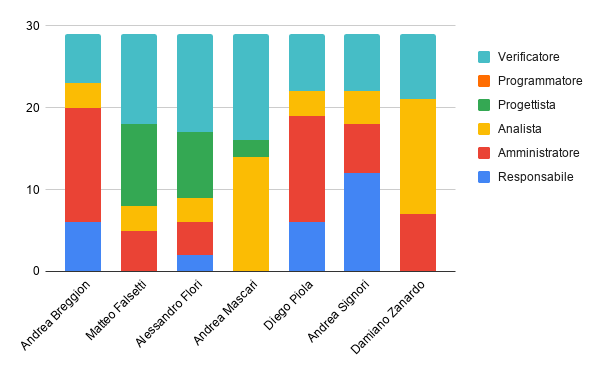
\includegraphics[width=0.8\textwidth]{source/img/analisi_orari.png}
        \caption{Divisione oraria dell'attività di analisi}
    \end{figure}
    \subsubsection{Prospetto economico}
    %startTable
    \def\salarycontent{
        {Amministratore,49,20,980},
        {Analista,44,25,1100},
        {Progettista,20,22,440},
        {Programmatore,0,15,0},
        {Responsabile,26,30,780},
        {Verificatore,64,15,960},
        {Totale,203,127,4260},
    }
    %endTable
    \newcommand*\salarysummary{}
\foreach \x [count=\nj] in \salarycontent
{
    \foreach \y [count=\ni] in \x
    {
        \ifnum\ni=1
            \xappto\salarysummary{\noexpand\textbf{\y}&}
        \else\ifnum\ni=3
            \xappto\salarysummary{\noexpand\euro\ \y&}
        \else\ifnum\ni=4
            \xappto\salarysummary{\noexpand\euro\ \y}
            \gappto\salarysummary{\\}
            \gappto\salarysummary{\hline} 
        \else
            \xappto\salarysummary{\y&}
        \fi\fi\fi
    }
}

% Impostazioni della tabella
\tabulinesep = 2mm % padding
\taburowcolors [1] 2{pari .. dispari} % colori delle righe
\begin{longtabu} to \textwidth {| X[0.1, c m] | X[0.1, c m] | X[0.1, c m] | X[0.1, c m] |}
\hline
\rowcolor{header} % colore dell'header
\textbf{Ruolo} &
\textbf{Ore} &
\textbf{Costo unitario (€)} & 
\textbf{Costo totale (€)} \\
\hline
\salarysummary
\end{longtabu}
\undef\salarysummary
    \begin{figure}[H]
        \centering
        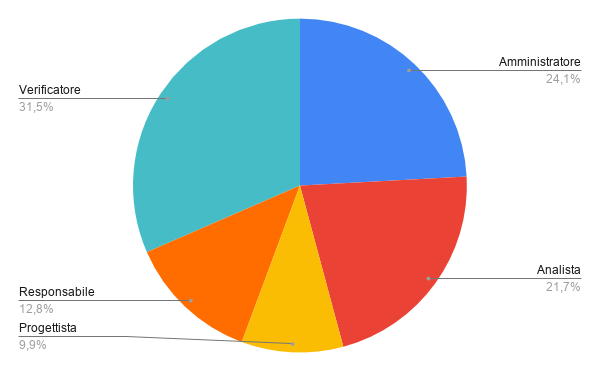
\includegraphics[width=0.8\textwidth]{source/img/analisi_ruoli.png}
        \caption{costo del personale nella fase di analisi}
    \end{figure}
\subsection{Consolidamento dei requisiti}
    \subsubsection{Prospetto orario}
    %startTable
    \def\hourlycontent{
        {Andrea Breggion,0,3,0,0,0,2,5},
        {Matteo Falsetti,0,0,0,1,0,4,5},
        {Alessandro Flori,0,0,0,1,0,4,5},
        {Andrea Mascari,0,0,5,0,0,0,5},
        {Diego Piola,2,0,3,0,0,0,5},
        {Andrea Signori,0,0,2,0,0,3,5},
        {Damiano Zanardo,0,0,5,0,0,0,5},
        {Ore totali,2,3,15,2,0,13,35},
    }
    %endTable
    \newcommand*\hourlysummary{}
\foreach \x [count=\nj] in \hourlycontent
{
    \foreach \y [count=\ni] in \x
    {
        \ifnum\ni=8
            \xappto\hourlysummary{\y}
            \gappto\hourlysummary{\\}
            \gappto\hourlysummary{\hline}
        \else
            \xappto\hourlysummary{\y&}
        \fi
    }
}

% Impostazioni della tabella
\tabulinesep = 2mm % padding
\taburowcolors [1] 2{pari .. dispari} % colori delle righe
\begin{longtabu} to \textwidth {| X[0.3, c m] | X[0.1, c m] | X[0.1, c m] | X[0.1, c m] | X[0.1, c m] | X[0.1, c m] | X[0.1, c m] | X[0.1, c m] |}
\hline
\rowcolor{header} % colore dell'header
\textbf{Membro} &
\textbf{Re} & 
\textbf{Ad} & 
\textbf{An} & 
\textbf{Pt} & 
\textbf{Pr} & 
\textbf{Ve} & 
\textbf{Ore totali} \\
\hline
\hourlysummary
\end{longtabu}
\undef\hourlysummary{} 
    \begin{figure}[H]
        \centering
        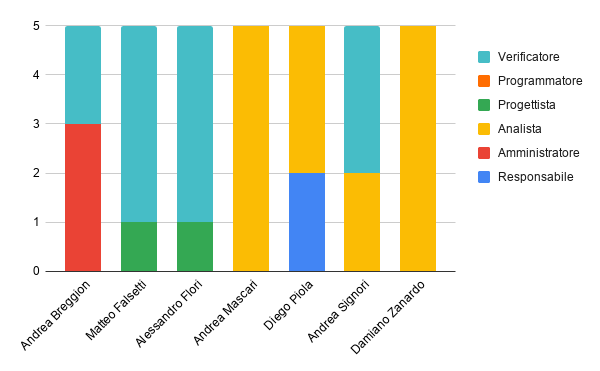
\includegraphics[width=0.8\textwidth]{source/img/consolidamento_orari.png}
        \caption{divisione oraria dell'attività di consolidamento dei requisiti}
    \end{figure}
    \subsubsection{Prospetto economico}
    %startTable
    \def\salarycontent{
        {Amministratore,3,20,60},
        {Analista,15,25,375},
        {Progettista,2,22,44},
        {Programmatore,0,15,0},
        {Responsabile,2,30,60},
        {Verificatore,13,15,195},
        {Totale,35,127,734},
    }
    %endTable
    \newcommand*\salarysummary{}
\foreach \x [count=\nj] in \salarycontent
{
    \foreach \y [count=\ni] in \x
    {
        \ifnum\ni=1
            \xappto\salarysummary{\noexpand\textbf{\y}&}
        \else\ifnum\ni=3
            \xappto\salarysummary{\noexpand\euro\ \y&}
        \else\ifnum\ni=4
            \xappto\salarysummary{\noexpand\euro\ \y}
            \gappto\salarysummary{\\}
            \gappto\salarysummary{\hline} 
        \else
            \xappto\salarysummary{\y&}
        \fi\fi\fi
    }
}

% Impostazioni della tabella
\tabulinesep = 2mm % padding
\taburowcolors [1] 2{pari .. dispari} % colori delle righe
\begin{longtabu} to \textwidth {| X[0.1, c m] | X[0.1, c m] | X[0.1, c m] | X[0.1, c m] |}
\hline
\rowcolor{header} % colore dell'header
\textbf{Ruolo} &
\textbf{Ore} &
\textbf{Costo unitario (€)} & 
\textbf{Costo totale (€)} \\
\hline
\salarysummary
\end{longtabu}
\undef\salarysummary
    \begin{figure}[H]
        \centering
        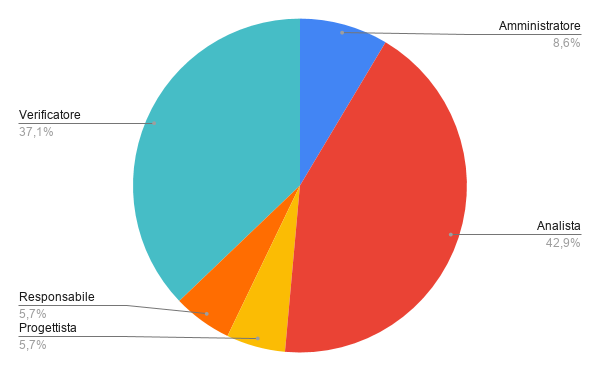
\includegraphics[width=0.8\textwidth]{source/img/consolidamento_ruoli.png}
        \caption{costo del personale nella fase di consolidamento dei requisiti}
    \end{figure}
\subsection{Progettazione architetturale}
    \subsubsection{Prospetto orario}
    %startTable
    \def\hourlycontent{
        {Andrea Breggion,0,7,4,6,5,4,26},
        {Matteo Falsetti,0,0,5,7,0,14,26},
        {Alessandro Flori,0,0,7,10,0,9,26},
        {Andrea Mascari,4,0,0,11,6,5,26},
        {Diego Piola,5,0,6,9,6,0,26},
        {Andrea Signori,0,6,4,7,5,4,26},
        {Damiano Zanardo,0,0,0,12,9,5,26},
        {Ore totali, 9, 13, 26, 62, 31, 41, 182},
    }
    %endTable
    \newcommand*\hourlysummary{}
\foreach \x [count=\nj] in \hourlycontent
{
    \foreach \y [count=\ni] in \x
    {
        \ifnum\ni=8
            \xappto\hourlysummary{\y}
            \gappto\hourlysummary{\\}
            \gappto\hourlysummary{\hline}
        \else
            \xappto\hourlysummary{\y&}
        \fi
    }
}

% Impostazioni della tabella
\tabulinesep = 2mm % padding
\taburowcolors [1] 2{pari .. dispari} % colori delle righe
\begin{longtabu} to \textwidth {| X[0.3, c m] | X[0.1, c m] | X[0.1, c m] | X[0.1, c m] | X[0.1, c m] | X[0.1, c m] | X[0.1, c m] | X[0.1, c m] |}
\hline
\rowcolor{header} % colore dell'header
\textbf{Membro} &
\textbf{Re} & 
\textbf{Ad} & 
\textbf{An} & 
\textbf{Pt} & 
\textbf{Pr} & 
\textbf{Ve} & 
\textbf{Ore totali} \\
\hline
\hourlysummary
\end{longtabu}
\undef\hourlysummary{}
    \begin{figure}[H]
        \centering
        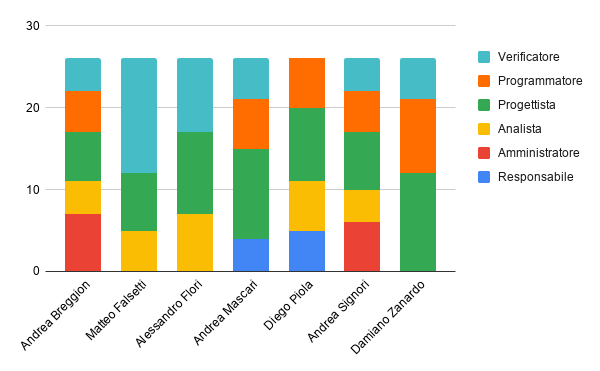
\includegraphics[width=0.8\textwidth]{source/img/architettura_orari.png}
        \caption{divisione oraria dell'attività di progettazione architetturale}
    \end{figure}
    \subsubsection{Prospetto economico}
    %startTable
    \def\salarycontent{
        {Amministratore,13,20,260},
        {Analista,26,25,650},
        {Progettista,62,22,1364},
        {Programmatore,31,15,465},
        {Responsabile,31,15,465},
        {Verificatore,41,15,615},
        {Totale,182,127,3624},
    }
    %endTable
    \newcommand*\salarysummary{}
\foreach \x [count=\nj] in \salarycontent
{
    \foreach \y [count=\ni] in \x
    {
        \ifnum\ni=1
            \xappto\salarysummary{\noexpand\textbf{\y}&}
        \else\ifnum\ni=3
            \xappto\salarysummary{\noexpand\euro\ \y&}
        \else\ifnum\ni=4
            \xappto\salarysummary{\noexpand\euro\ \y}
            \gappto\salarysummary{\\}
            \gappto\salarysummary{\hline} 
        \else
            \xappto\salarysummary{\y&}
        \fi\fi\fi
    }
}

% Impostazioni della tabella
\tabulinesep = 2mm % padding
\taburowcolors [1] 2{pari .. dispari} % colori delle righe
\begin{longtabu} to \textwidth {| X[0.1, c m] | X[0.1, c m] | X[0.1, c m] | X[0.1, c m] |}
\hline
\rowcolor{header} % colore dell'header
\textbf{Ruolo} &
\textbf{Ore} &
\textbf{Costo unitario (€)} & 
\textbf{Costo totale (€)} \\
\hline
\salarysummary
\end{longtabu}
\undef\salarysummary
    \begin{figure}[H]
        \centering
        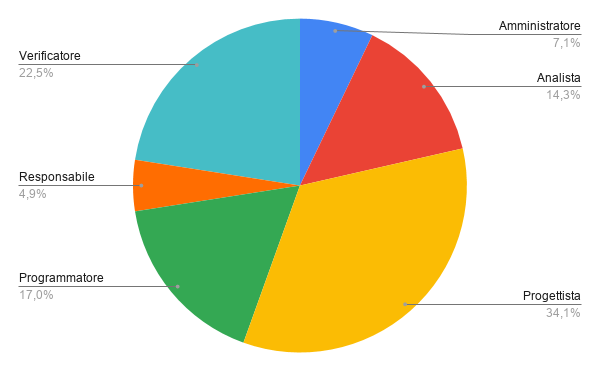
\includegraphics[width=0.8\textwidth]{source/img/architettura_ruoli.png}
        \caption{costo del personale nella fase di progettazione architetturale}
    \end{figure}
\subsection{Progettazione di dettaglio e codifica}
    \subsubsection{Prospetto orario}
    %startTable
    \def\hourlycontent{
        {Andrea Breggion,5,6,0,7,20,10,48},
        {Matteo Falsetti,5,0,0,15,15,13,48},
        {Alessandro Flori,0,4,0,10,18,16,48},
        {Andrea Mascari,0,0,0,14,22,12,48},
        {Diego Piola,5,6,0,9,20,8,48},
        {Andrea Signori,0,0,0,13,22,13,48},
        {Damiano Zanardo,0,6,0,12,20,10,48},
        {Ore totali, 15, 22, 0, 80, 137, 82, 336},
    }
    %endTable
    \newcommand*\hourlysummary{}
\foreach \x [count=\nj] in \hourlycontent
{
    \foreach \y [count=\ni] in \x
    {
        \ifnum\ni=8
            \xappto\hourlysummary{\y}
            \gappto\hourlysummary{\\}
            \gappto\hourlysummary{\hline}
        \else
            \xappto\hourlysummary{\y&}
        \fi
    }
}

% Impostazioni della tabella
\tabulinesep = 2mm % padding
\taburowcolors [1] 2{pari .. dispari} % colori delle righe
\begin{longtabu} to \textwidth {| X[0.3, c m] | X[0.1, c m] | X[0.1, c m] | X[0.1, c m] | X[0.1, c m] | X[0.1, c m] | X[0.1, c m] | X[0.1, c m] |}
\hline
\rowcolor{header} % colore dell'header
\textbf{Membro} &
\textbf{Re} & 
\textbf{Ad} & 
\textbf{An} & 
\textbf{Pt} & 
\textbf{Pr} & 
\textbf{Ve} & 
\textbf{Ore totali} \\
\hline
\hourlysummary
\end{longtabu}
\undef\hourlysummary{}
    
    \begin{figure}[H]
        \centering
        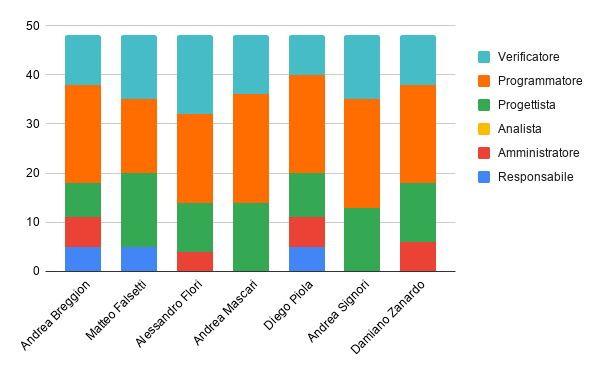
\includegraphics[width=0.8\textwidth]{source/img/codifica_orari.png}
        \caption{divisione oraria dell'attività di progettazione di dettaglio e codifica}
    \end{figure}
    \subsubsection{Prospetto economico}
    %startTable
    \def\salarycontent{
        {Amministratore,22,20,440},
        {Analista,0,25,0},
        {Progettista,80,22,1760},
        {Programmatore,137,15,2055},
        {Responsabile,15,30,450},
        {Verificatore,82,15,1230},
        {Totale,336,127,5935},
    }
    %endTable
    \newcommand*\salarysummary{}
\foreach \x [count=\nj] in \salarycontent
{
    \foreach \y [count=\ni] in \x
    {
        \ifnum\ni=1
            \xappto\salarysummary{\noexpand\textbf{\y}&}
        \else\ifnum\ni=3
            \xappto\salarysummary{\noexpand\euro\ \y&}
        \else\ifnum\ni=4
            \xappto\salarysummary{\noexpand\euro\ \y}
            \gappto\salarysummary{\\}
            \gappto\salarysummary{\hline} 
        \else
            \xappto\salarysummary{\y&}
        \fi\fi\fi
    }
}

% Impostazioni della tabella
\tabulinesep = 2mm % padding
\taburowcolors [1] 2{pari .. dispari} % colori delle righe
\begin{longtabu} to \textwidth {| X[0.1, c m] | X[0.1, c m] | X[0.1, c m] | X[0.1, c m] |}
\hline
\rowcolor{header} % colore dell'header
\textbf{Ruolo} &
\textbf{Ore} &
\textbf{Costo unitario (€)} & 
\textbf{Costo totale (€)} \\
\hline
\salarysummary
\end{longtabu}
\undef\salarysummary
    \begin{figure}[H]
        \centering
        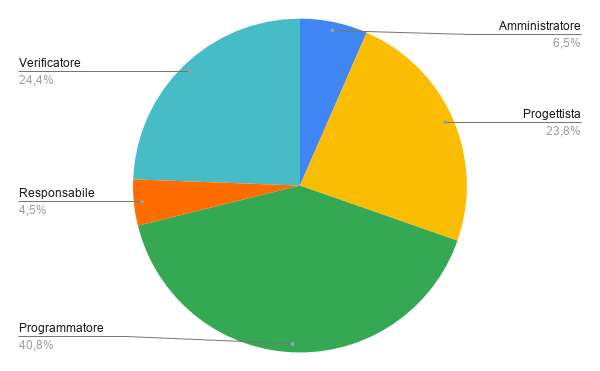
\includegraphics[width=0.8\textwidth]{source/img/codifica_ruoli.png}
        \caption{costo del personale nella fase di progettazione di dettaglio e codifica}
    \end{figure}
\subsection{Validazione e collaudo}
    \subsubsection{Prospetto orario}
    %startTable
    \def\hourlycontent{
        {Andrea Breggion,0,5,0,5,8,8,26},
        {Matteo Falsetti,0,5,0,10,5,6,26},
        {Alessandro Flori,5,0,0,7,4,10,26},
        {Andrea Mascari,0,6,0,6,5,9,26},
        {Diego Piola,0,0,0,8,8,10,26},
        {Andrea Signori,4,0,0,6,9,7,26},
        {Damiano Zanardo,6,0,0,6,4,10,26},
        {Ore totali,15,16,0,48,43,60,182},
    }
    %endTable
    \newcommand*\hourlysummary{}
\foreach \x [count=\nj] in \hourlycontent
{
    \foreach \y [count=\ni] in \x
    {
        \ifnum\ni=8
            \xappto\hourlysummary{\y}
            \gappto\hourlysummary{\\}
            \gappto\hourlysummary{\hline}
        \else
            \xappto\hourlysummary{\y&}
        \fi
    }
}

% Impostazioni della tabella
\tabulinesep = 2mm % padding
\taburowcolors [1] 2{pari .. dispari} % colori delle righe
\begin{longtabu} to \textwidth {| X[0.3, c m] | X[0.1, c m] | X[0.1, c m] | X[0.1, c m] | X[0.1, c m] | X[0.1, c m] | X[0.1, c m] | X[0.1, c m] |}
\hline
\rowcolor{header} % colore dell'header
\textbf{Membro} &
\textbf{Re} & 
\textbf{Ad} & 
\textbf{An} & 
\textbf{Pt} & 
\textbf{Pr} & 
\textbf{Ve} & 
\textbf{Ore totali} \\
\hline
\hourlysummary
\end{longtabu}
\undef\hourlysummary{}
    \begin{figure}[H]
        \centering
        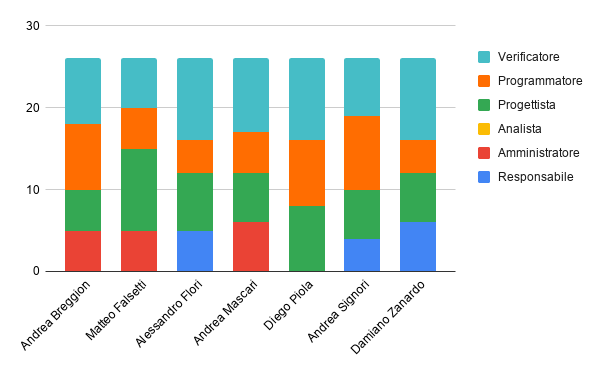
\includegraphics[width=0.8\textwidth]{source/img/validazione_orari.png}
        \caption{divisione oraria dell'attività di validazione e collaudo}
    \end{figure}
    \subsubsection{Prospetto economico}
    %startTable
    \def\salarycontent{
        {Amministratore,16,20,320},
        {Analista,0,25,0},
        {Progettista,48,22,1056},
        {Programmatore,43,15,645},
        {Responsabile,15,30,450},
        {Verificatore,60,15,900},
        {Totale,182,127,3371},
    }
    %endTable
    \newcommand*\salarysummary{}
\foreach \x [count=\nj] in \salarycontent
{
    \foreach \y [count=\ni] in \x
    {
        \ifnum\ni=1
            \xappto\salarysummary{\noexpand\textbf{\y}&}
        \else\ifnum\ni=3
            \xappto\salarysummary{\noexpand\euro\ \y&}
        \else\ifnum\ni=4
            \xappto\salarysummary{\noexpand\euro\ \y}
            \gappto\salarysummary{\\}
            \gappto\salarysummary{\hline} 
        \else
            \xappto\salarysummary{\y&}
        \fi\fi\fi
    }
}

% Impostazioni della tabella
\tabulinesep = 2mm % padding
\taburowcolors [1] 2{pari .. dispari} % colori delle righe
\begin{longtabu} to \textwidth {| X[0.1, c m] | X[0.1, c m] | X[0.1, c m] | X[0.1, c m] |}
\hline
\rowcolor{header} % colore dell'header
\textbf{Ruolo} &
\textbf{Ore} &
\textbf{Costo unitario (€)} & 
\textbf{Costo totale (€)} \\
\hline
\salarysummary
\end{longtabu}
\undef\salarysummary
    \label{image:verifica_ruoli}
    \begin{figure}[H]
        \centering
        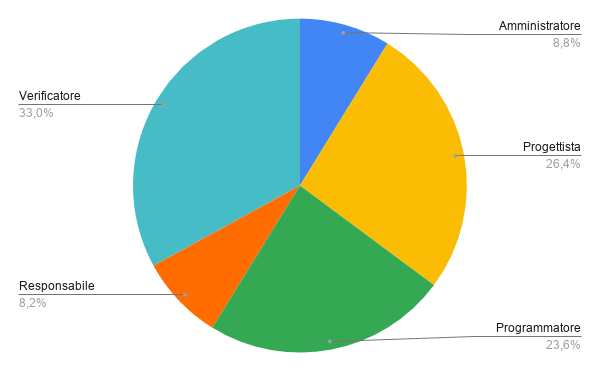
\includegraphics[width=0.8\textwidth]{source/img/validazione_ruoli.png}
        \caption{costo del personale nella fase di validazione e collaudo}
    \end{figure}
\subsection{Riepilogo}
    \subsection{Ore totali}
    All'interno di questa sottosezione è contenuto il riepilogo delle ore totali, comprensive dell'investimento, che non sarà rendicontato nell'offerta finale, ossia della fase di analisi.
        \paragraph{Suddivisione del lavoro}
        
        %startTable
        \def\hourlycontent{
            {Andrea Breggion,11,35,7,18,33,30,134},
            {Matteo Falsetti,5,10,8,43,20,48,134},
            {Alessandro Flori,7,8,10,36,22,51,134},
            {Andrea Mascari,4,6,19,33,33,39,134},
            {Diego Piola,18,19,12,26,34,25,134},
            {Andrea Signori,16,12,10,26,36,34,134},
            {Damiano Zanardo,6,13,19,30,33,33,134},
            {Ore totali,67,103,85,212,211,260,938},
        }
        %endTable
        \newcommand*\hourlysummary{}
\foreach \x [count=\nj] in \hourlycontent
{
    \foreach \y [count=\ni] in \x
    {
        \ifnum\ni=8
            \xappto\hourlysummary{\y}
            \gappto\hourlysummary{\\}
            \gappto\hourlysummary{\hline}
        \else
            \xappto\hourlysummary{\y&}
        \fi
    }
}

% Impostazioni della tabella
\tabulinesep = 2mm % padding
\taburowcolors [1] 2{pari .. dispari} % colori delle righe
\begin{longtabu} to \textwidth {| X[0.3, c m] | X[0.1, c m] | X[0.1, c m] | X[0.1, c m] | X[0.1, c m] | X[0.1, c m] | X[0.1, c m] | X[0.1, c m] |}
\hline
\rowcolor{header} % colore dell'header
\textbf{Membro} &
\textbf{Re} & 
\textbf{Ad} & 
\textbf{An} & 
\textbf{Pt} & 
\textbf{Pr} & 
\textbf{Ve} & 
\textbf{Ore totali} \\
\hline
\hourlysummary
\end{longtabu}
\undef\hourlysummary{} 
        \begin{figure}[H]
            \centering
            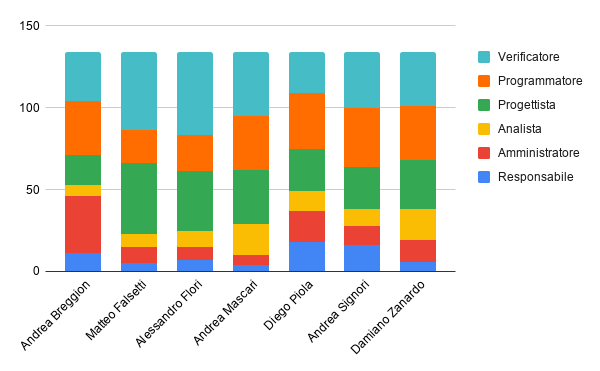
\includegraphics[width=0.8\textwidth]{source/img/totale_orari.png}
            \caption{divisione oraria complessiva}
        \end{figure}
        \paragraph{Prospetto economico}
        
        %startTable
        \def\salarycontent{
            {Amministratore,103,20,2060},
            {Analista,85,25,2125},
            {Progettista,212,22,4664},
            {Programmatore,211,15,3165},
            {Responsabile,67,30,2010},
            {Verificatore,260,15,3900},
            {Totale,938,127,17924},
        }
        %endTable
        \newcommand*\salarysummary{}
\foreach \x [count=\nj] in \salarycontent
{
    \foreach \y [count=\ni] in \x
    {
        \ifnum\ni=1
            \xappto\salarysummary{\noexpand\textbf{\y}&}
        \else\ifnum\ni=3
            \xappto\salarysummary{\noexpand\euro\ \y&}
        \else\ifnum\ni=4
            \xappto\salarysummary{\noexpand\euro\ \y}
            \gappto\salarysummary{\\}
            \gappto\salarysummary{\hline} 
        \else
            \xappto\salarysummary{\y&}
        \fi\fi\fi
    }
}

% Impostazioni della tabella
\tabulinesep = 2mm % padding
\taburowcolors [1] 2{pari .. dispari} % colori delle righe
\begin{longtabu} to \textwidth {| X[0.1, c m] | X[0.1, c m] | X[0.1, c m] | X[0.1, c m] |}
\hline
\rowcolor{header} % colore dell'header
\textbf{Ruolo} &
\textbf{Ore} &
\textbf{Costo unitario (€)} & 
\textbf{Costo totale (€)} \\
\hline
\salarysummary
\end{longtabu}
\undef\salarysummary
        \begin{figure}[H]
            \centering
            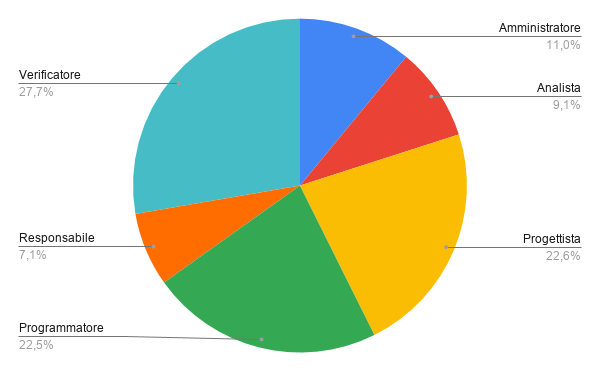
\includegraphics[width=0.8\textwidth]{source/img/totale_ruoli.png}
            \caption{costo del personale complessivo}
        \end{figure}
    \subsection{Ore rendicontate}
    All'interno di questa sottosezione è contenuto il riepilogo delle ore dedicate all'attività di progetto nonché il riepilogo dei costi relativi al periodo successivo alla RR.
        \paragraph{Suddivisione del lavoro}
        
        %startTable
        \def\hourlycontent{
            {Andrea Breggion,5,21,4,18,33,24,105},
            {Matteo Falsetti,5,5,5,33,20,37,105},
            {Alessandro Flori,5,4,7,28,22,39,105},
            {Andrea Mascari,4,6,5,31,33,26,105},
            {Diego Piola,12,6,9,26,34,18,105},
            {Andrea Signori,4,6,6,26,36,27,105},
            {Damiano Zanardo,6,6,5,30,33,25,105},
            {Ore totali,41,54,41,192,211,196,735},
        }
        %endTable
        \newcommand*\hourlysummary{}
\foreach \x [count=\nj] in \hourlycontent
{
    \foreach \y [count=\ni] in \x
    {
        \ifnum\ni=8
            \xappto\hourlysummary{\y}
            \gappto\hourlysummary{\\}
            \gappto\hourlysummary{\hline}
        \else
            \xappto\hourlysummary{\y&}
        \fi
    }
}

% Impostazioni della tabella
\tabulinesep = 2mm % padding
\taburowcolors [1] 2{pari .. dispari} % colori delle righe
\begin{longtabu} to \textwidth {| X[0.3, c m] | X[0.1, c m] | X[0.1, c m] | X[0.1, c m] | X[0.1, c m] | X[0.1, c m] | X[0.1, c m] | X[0.1, c m] |}
\hline
\rowcolor{header} % colore dell'header
\textbf{Membro} &
\textbf{Re} & 
\textbf{Ad} & 
\textbf{An} & 
\textbf{Pt} & 
\textbf{Pr} & 
\textbf{Ve} & 
\textbf{Ore totali} \\
\hline
\hourlysummary
\end{longtabu}
\undef\hourlysummary{}
        \begin{figure}[H]
            \centering
            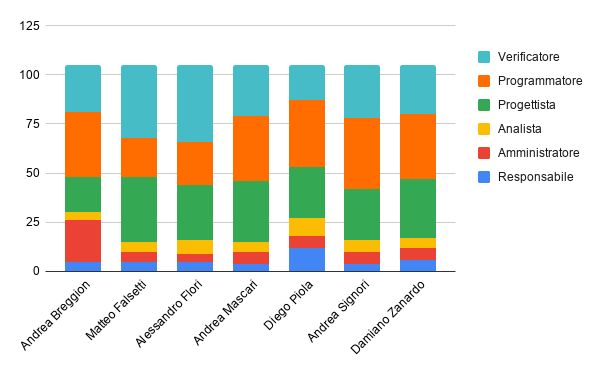
\includegraphics[width=0.8\textwidth]{source/img/no_investimento_orari.png}
            \caption{divisione oraria totale senza l'investimento iniziale}
        \end{figure}
        \paragraph{Prospetto economico}
        
        %startTable
        \def\salarycontent{
            {Amministratore,54,20,1080},
            {Analista,41,25,1025},
            {Progettista,192,22,4224},
            {Programmatore,211,15,3165},
            {Responsabile,41,30,1230},
            {Verificatore,196,15,2940},
            {Totale,735,127,13664},
        }
        %endTable
        \newcommand*\salarysummary{}
\foreach \x [count=\nj] in \salarycontent
{
    \foreach \y [count=\ni] in \x
    {
        \ifnum\ni=1
            \xappto\salarysummary{\noexpand\textbf{\y}&}
        \else\ifnum\ni=3
            \xappto\salarysummary{\noexpand\euro\ \y&}
        \else\ifnum\ni=4
            \xappto\salarysummary{\noexpand\euro\ \y}
            \gappto\salarysummary{\\}
            \gappto\salarysummary{\hline} 
        \else
            \xappto\salarysummary{\y&}
        \fi\fi\fi
    }
}

% Impostazioni della tabella
\tabulinesep = 2mm % padding
\taburowcolors [1] 2{pari .. dispari} % colori delle righe
\begin{longtabu} to \textwidth {| X[0.1, c m] | X[0.1, c m] | X[0.1, c m] | X[0.1, c m] |}
\hline
\rowcolor{header} % colore dell'header
\textbf{Ruolo} &
\textbf{Ore} &
\textbf{Costo unitario (€)} & 
\textbf{Costo totale (€)} \\
\hline
\salarysummary
\end{longtabu}
\undef\salarysummary
        \begin{figure}[H]
            \centering
            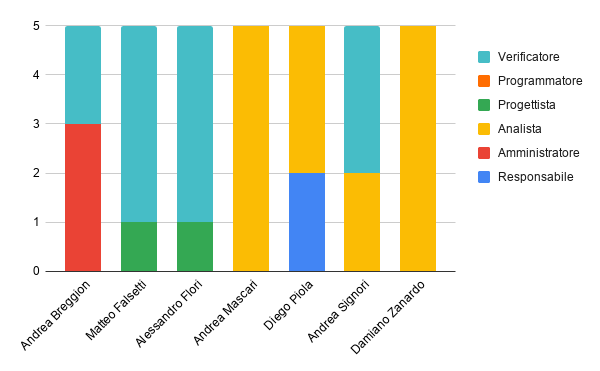
\includegraphics[width=0.8\textwidth]{source/img/consolidamento_orari.png}
            \caption{costo totale del personale senza l'investimento iniziale}
        \end{figure}
    \subsection{Conclusioni}
    All'interno della tabella di cui sopra è indicata l'offerta con cui Code of Duty si presenta al committente. Tale somma ammonta a \euro\ 13664.

    
\end{document}